%%%%%%%%%%%%%%%%%%%%%%%%%%%%%%%%%%%%%%%%%%%%%%%%%%%%%%%%%%%%%%%
%
% Welcome to Overleaf --- just edit your LaTeX on the left,
% and we'll compile it for you on the right. If you open the
% 'Share' menu, you can invite other users to edit at the same
% time. See www.overleaf.com/learn for more info. Enjoy!
%
%%%%%%%%%%%%%%%%%%%%%%%%%%%%%%%%%%%%%%%%%%%%%%%%%%%%%%%%%%%%%%%
\documentclass{article}
\usepackage[english]{babel}
\usepackage{indentfirst}
\usepackage{float}
\usepackage{listings}
\usepackage{graphics}
\usepackage[colorlinks=true, urlcolor = blue,citecolor = black,]{hyperref}
% \usepackage[letterpaper,top=2cm,bottom=2cm,left=3cm,right=3cm,marginparwidth=2cm]{geometry}
\usepackage{fullpage} 
\usepackage{pgfplots}
\usepackage{amsmath} 
\pgfplotsset{width=10cm,compat=1.5}
\setlength{\arrayrulewidth}{0.25mm}

\setlength{\tabcolsep}{10pt}
\renewcommand{\arraystretch}{1}
\title{Analysis of Naive Bayes Based Spam Filter with Different N-Gram }
\author{Zirui Chen}

\begin{document}
\maketitle

\begin{abstract}
Unsolicited emails are growing into one of the biggest threats to all users. It is estimated that over 85 percent\cite{Cveticanin} of email sent daily are unsolicited emails. Various methods have been developed to identify unsolicited emails, including but not limited to machine learning based algorithms, traffic tracking methods and white-black lists. The naive bayes classifier incorporated with natural language processing techniques and large training data sets might improve the performance of spam filters. Two correctional experiments are conducted where unigram, bigram, and trigram are integrated with naive bayes classifier. The bigram version of this spam filter is also trained with a larger data set in order to validate the hypothesis that performance can be effected by the size of training data. Statistics, namely percision, recall, F-score and accuracy, are recorded and analyzed. Normal naive bayes classifier with unigram achieved 92.15 \% overall accuracy. Normal naive bayes classifier with bigram achieved 93.59\%  accuracy and trigram version of this spam filter achieved 90.79\% accuracy. Bigram spam filters trained with larger data achieve 94.28\% accuracy, which is 0.69\% higher than normal bigram spam filters. As result, we can conclude that natural language processing techniques can play a major role in improving the accuracy of spam filters. Also, results validate that spam filters will have better performance with larger training data size. 
\end{abstract}
\section{Introduction}


With the rapid development of the internet comes the rapid increase of spam messages. Spam messages, as defined by the Merriam Webster dictionary, are unsolicited commercial messages sent to a large number of recipients or posted in a large number of places. It is estimated that over 85 percent of email sent worldwide should be categorized as spam messages\cite{Cveticanin}. 


There are two main types of spam messages\cite{"Arutyunov"}. The most common and probably less harmful type are the ones that prompt products. Such messages usually contain the description about the product, some promotion messages contain links or phone numbers towards the seller. The other more harmful kind of spam messages usually have malice intent. Such messages usually have different formats with different maleficent intent. For example, some spam messages categorized as phishing emails will try to obtain sensitive information from users. Some messages have spyware encoded in the mail. Once the mail is opened and/or some content is downloaded, all user’s activity and sensitive information will be sent to spammers. Based on recent research, the losses to individuals and businesses caused by spam emails has an yearly estimated of 4.2 billion\cite{FBI}.


Spam filters are keen to save users time and decrease the loss caused by spam. There exit various methods that target some parts of the message to differentiate spam messages from usual correspondence, namely content filter, header filter, block filter and rules-based filter. Various implementations of content based spam filter have been proposed, such as machine learning based algorithms, black -list and white-list filtering and support vector machine filtering. As the fast development and deployment of spam filters, the spammers are also rapidly adapting. Identifying spam messages from the rest of messages would be a challenging task since the format of spam messages varies.There are many counter measures that the spammers have developed in order to infiltrate and disable spam filters. The most naive and common approach is to guise spam messages as normal correspondences. There exists some more sophisticated approaches. For example, a technique called data poisoning could be deployed if spammers are trying to disable machine learning based algorithms. The idea behind data poisoning is to provide false data to the training set. Such action could, from its root, jeopardize the model created. The ideal outcome is that the spam filters are no longer effective towards certain types of spam messages. 
 
 
Due to the importance of spam filters, developers must use extreme caution when implementing spam filters since any misjudgement can cause great harm. For example, it must be noted that we should be extremely careful when we want to classify certain emails as spam and put them into a spam folder since one misclassified ham message can cause more harm than 100 misclassified spam messages.


For the purpose of increasing overall accuracy of general naive bayes based spam filtering, we decided to introduce natural language processing techniques into the feature extraction step of building a machine learning model. Instead of the normal unigram method, bigram and trigram with back fire and/or good turing smoothing will be used and the result will be compared. This work provides mean to validate the assumption that natural language processing techniques can increase the overall accuracy of naive bayes based spam filters. Furthermore, this article will conduct experiments on how the size and length of the training set could affect the performance of spam filters. Ergo, the main purpose of this article is to validate the hypothesis that natural language processing can be used to increase the accuracy of the spam filter and the size of the training set could greatly influence the performance of the spam filter created. 


This article is organized as follows. A thorough literature review will be conducted in the background section. Plan will be detailed in the approach section. Experimental design and experimental results will be presented in the experiment and result section. Results will be analyzed and discussed in the analysis section. Conclusion describes the overall finding and results derived from the findings. On top of that, future research is also described in the conclusion section. 
\section{Background}


Morden spam filtering techniques can be generally categorized into two categories, namely reputation based filtering and content-based filtering.\cite{Bhowmick} Reputation based filtering can be further categorized as origin based, social networks, traffic analysis and protocol based filtering. Content-based filtering can also be further categorized as heuristics fingerprint based and machine learning based.


Black-list and white-lsit is one widely adopted method of reputation based filtering. The idea is to set up a Real time IP address balck-list. \cite{Bhowmick}Every Time user receives a message, the filter will firstly compare the IP address of the sender with IPs in balck-list. If there is a match, the email will be automatically sent to trash. However, this technique is inherently flawed since there are many ways to get around it. One of the techniques is the use of botNets. Botnets are capable of sending massive amounts of spam messages with different IP addresses. This will significantly increase the number of IP addresses on the black-list. On the other hand, putting messages into the trash without taking a look at the content will increase the odds of false positives. False positives in this case means that legit messages are wrongfully categorized as spam messages. The cost of having false positives is much more expensive than false negatives.


Another approach under reputation-based filtering is traffic analysis.\cite{Zhang} Under the presumption that spam emails from one spammer usually have the same content, messages can then be categorized under the similarity of message content. If one category has lots of similar messages, a method can be applied to filter such messages. One method used during the IEEE 2006 conference is called Bulk Mil Traffic Classification. The result indicates that it has a 70.4 percent accurate rate to filter out spam mails in a fast and cheap manner. 
Content-based filters are believed to be the method that can achieve the highest accuracy. In morden machine learning based content filters, various machine learning techniques are used in combination with natural language processing techniques. Before any machine learning methods can be applied, data must be tokenized, stemmed and cleaned. Several natural language processing techniques can be used to help feature extraction, which would significantly increase accuracy. 


The most commonly used content-based filtering method is Bayesian classifier. This classifier method implements a statistical method called maximum posteriori probability(MAP).\cite{Khorsi} Firstly, we need to obtain a data set, which should clearly indicate the data type( spam or ham). Secondly, the data set should be randomly split to 20 percent:80 percent. The 80 percent shall be used as the training set and 20 percent as the test set. Bayesian can then be used to classify the data in a training set. The model shall be tested using the test data. Results should be evaluated by four scores, namely Precision, F-score,recall and accuracy.\cite{Muhammad} As discussed earlier, NLP can play an important role in feature extraction. There are several approaches such as the N-gram model\cite{tunga}, pos tagging and message entropy.\cite{Ezpeleta}The bayesian classifier can be fed with data that is processed by different MPL methods to achieve a better model. The Bayesian classification has an accuracy of over 95percent when properly implemented. However, it is also subject to many vulnerabilities such as bayesian poisoning. The idea behind bayesian poisoning is to poison the model by feeding the classifier wrongfully marked data(e.g. Sending legit messages and reporting them as spam).\cite{Blanzieri} 


Another simple approach of content-based filtering is called k nearest neighbors.\cite{Khorsi} The idea is roughly the same as the Bayesian classifier, the only difference is that the modeling process. This algorithm has a predefined number of centers, and the center will be automatically updated based on the data. Once modeling is completed, an outgoing message will be evaluated, if a large portion of it is in k neighborhood, then it would be categorized as spam. 


One of the most recent techniques is called a support vector machine. A support vector machine is a framework that minimizes risk.\cite{Subramaniam} It’s developed by Vapnik based on optimal classification.  This framework, in its essence, is to find a hyperplane that separates spam and ham classes. Under the circumstance that the datas are not linearly spepartelable, the hyperplane will be found in higher dimensions.\cite{Khorsi} This framework is deemed to be efficient and accurate. 


One natural language processing technique used for spam detection is called maximum entropy. Entropy means the amount of information composted in a piece of information. The idea is to find the “appropriate probability distribution that maximizes the entropy”.\cite{Khorsi}
We must note that in morden spam detection systems, all aforementioned techniques work together, in whole or in parts, to ensure the best accuracy of spam detection. To deliver the state of the art spam filter would require millions of data and years of effort. My project would focus on how different NLP processing techniques would affect the accuracy of sample machine learning classification.


The size of the data set and length of message is keen to the model in training. In this article, we will also conduct experiments on that front. 
\section{Approach}
The general idea is to process the data with unigram, bigram and trigram method. Then choose a different training set and testing set ratio with different N-gram models. Run each combination through the classification function. After the model has been trained, we will run all test data through a predict function and keep track of the numbers. Statistics will be reported at the end of the program. Analysis of data reported will be conducted. 

To be more specific,a data set of tagged messages will be collected. Data will be firstly randomly separated into two portions, one as the training set and another as the test set. The ration between training data and test data will be set to 8 to 2. After the data is separated, spam messages and ham messages will be separated into two lists, namely spam and ham. Then, all messages will be processed by natural language processing methods. 


The N-gram method is deployed to process such messages. Unigram, bigram and trigram will be used in the effort to increase the overall accuracy of spam filters. In this context, unigram means that all words in a sentence will be separated one by one. Bigram means that words will be separated two by two and trigram means that words will be separated three by three. With such implementation, there is a possibility that we will encounter tokens that we have never met before. On top of that, there is a high possibility that we will encounter words that are out of dictionary. In order to overcome such problems, a statistical technique called good-turing frequency estimation will be implemented. By using good-turing frequency estimation, we can obtain the estimated probability of this token with the token we have seen before\cite{Avasthi}. 


To implement such concepts, firstly, we must turn all words into lowercase letters. Secondly, all sentences shall be processed by unigram, bigram and trigram methods in the NLTK library. Thirdly, all those tokens should be stored in a dictionary and the term frequency-inverse document frequency shall be calculated via 
\[(1+log f_t_,_d)\times log(\frac{N}{n_t})\]
where N is the total number of words, \(n_t\) is the number of frequencies of a certain word token and \(f_t_,_q\) is the frequency of a certain work token in the context. 


The good turing frequency estimation is calculated through this function:

\[\frac{(r+1)S(N_r_+_1)}{N}\]
Where r the number of times such patterns have been seen.  \(N_r_+_1\) is the number of words that’s in the data set which contains the r+1 number of times such patterns have been seen. \(N_r\) is the number of words that’s in the data set which contains the r number of times such patterns have been seen.


Then, use the simple naive bayes as means to build models. The formula for naive bayes is listed as follows:
\[p(C_k|x)=\frac{P(C_K)p(x|C_k)}{p(x)}\]
the \(P(C_k|x)\) is the posterior. \(P(C_k)\) is the prior. \(p(x|C_k)\) is the likelihood and \(p(x)\) is the evidence.

 
Algorithm is described as follows\cite{"Karmali"}. 
\begin{lstlisting}[language=Python,]
    def classify:
        pSpam, pHam = 0
        for word in processed_message:                
            if word in self.prob_spam:
                pSpam += log(self.prob_spam[word])
            else:
                pSpam -= log(self.sum_tf_idf_spam + len(list(self.prob_spam.keys())))
            if word in self.prob_ham:
                pHam += log(self.prob_ham[word])
            else:
                pHam -= log(self.sum_tf_idf_ham + len(list(self.prob_ham.keys())))  
            pSpam += log(self.prob_spam_mail)
            pHam += log(self.prob_ham_mail)
        return pSpam >= pHam

\end{lstlisting}


Once model building is completed, we could run a testing set through predict function and calculator metric, namely precision, recall,F-score and accuracy based on the prediction and the tags. 


Precision is used to describe how accurately we can correctly classify some message among all messages with the same tag.  Precision is calculated as the number of true positives divided by the sum of true positives and false positives. The equation for this calculation is:
\[Precision=\frac{true positive}{true positives+false positives}\]


Recall is used to describe how accurately this model can identify true positives among all samples.Recall is calculated as the number of the true positives divided by the sun of the true positive and false negatives. The equation for this calculation is:

\[Recall=\frac{true positive}{true positives+false negatives}\]

F-score is the combination of recall and precision. Such a metric will make comparison between models easier to understand. F-score is calculated as the product of precision and recall times two divided by the sum of precision and recall. The equation for this calculation is:

\[F-score=\frac{2\times Precision\times Recall}{Precision+Recall}\]


Accuracy is used to examine the overall accuracy of classification. Accuracy is calculated as the the sum of true positive and true negative divided by the sum of true positives, true negative, false negative and false positive. The equation for this calculation is:
\[Accuracy=\frac{true positive+true negatives}{true positives+true negatives+false negatives+false positives}\]

Since the training set and testing set is randomly chosen, the prediction is deemed to have a non deterministic behavior. Ten runs will be conducted for unigram, bigram and trigrams and the metrics will be recorded. The means then will be calculated and analyzed. 


In order to establish that the size of the data set has a significant effect on the model build and spam filter. We can simulate this by giving more data to the train set and less data to the test set. We will then turn the training data and test date ratio into 9 to 1. Then run the program with biigram ten times and keep the results recorded. Compare the bigram spam filter with more training data with the normal bigram spam filter. The average shall be calculated for feature analysis. 

\section{Experimental design and results:}
This study follows the principle of correlational study. The idea of correlation study is to observe the relationship between two sets of variables better. All experiments will use the same program\footnotemark[1] with little difference. There are two sets of experiments with three sets of variables. The first set of experiments is to test which n grams can produce the best overall statistics using the same database at 2:8 ratio. We will record the performance, namely precision, recall, F-score and accuracy, for unigram implementation, bigram implementation and trigram implementation. The results will be analyzed. 

\footnotetext[1]{the source for this program is firstly obtained through \href{https://github.com/tejank10/Spam-or-Ham}{Tejan Karmali's github Spam-or-Ham}. modifications have been made including but not limited to n-grams, good-turing smoothing}
The second set of experiments is to test whether the size of the training set could cause differences in overall performance. Bigram model will be used in this implementation. For the control group, the training set to test set ratio will be kept at 2 to 8. For the other group, the training set: test set ratio will be set to  1 to 9. We will record the performance, namely precision, recall, F-score and accuracy, for unigram implementation, bigram implementation and trigram implementation. The results will be analyzed. 

The classify spam message database is obtained through kaggle. There are 5169 unique tag messages. Among 5169, 87 percent of the messages are tagged as ham messages and 13 percent of them are tagged as spam messages. The average length of mail messages is 20 words while the shortest message length is 3 and longest message length is 78. 


Classified spam message data is stored in a csv file. Firstly, we use the pandas library to read in this csv file. After the file is processed, we must pre-process the input data by dropping unneeded columbus and rename the first column(tags) as labels and second column as messages. Then, turn all labels into 0 or 1 where 1 stands for han and 1 stands for spam. After the pre-process is completed, a numpy uniform method is used to randomly choose the training set and testing set. The interval is set to 0 and 1. Under the assumption that the number will be randomly generated, data which obtains less than 80 will be categorized as the training data and data which obtain more or equal to 80 will be categorized as the testing data. We will split the training set and testing set into two different numpy lists. This approach is feasible since the difference is no larger than 3 for most cases. Once such separation is completed, we will firstly turn all words into stem. In natural language processing, steam is the form of a word before and inflectional affixes are added. After all words turned into stem words, all stop words will be firstly removed. Stop words are defined as the words that do not bear any useful meaning such as i, me, the. After, a different N-gram method will be applied to all messages using NLTK library methods. Word tokens will be stored in a list. Then, calculate term frequency and inverse document frequency based on the equation described in the approach section. After model building is completed, we will run all messages in the test data set through the predict function. The prediction data will be collected and statistics will be produced. 


Due to the non deterministic behavior of this program, 10 test runs will be conducted for each implementation and results will be recorded. Average will also calculated based on the date recorded. Then charts will be generated for each of the metrics for further analysis. 
In order to validate the hypothesis that the size of training data and length of training data could impact the model build. One extra test run that implements the bigram model will be conducted. As usual, all data will be recorded and average will also be calculated for further analysis. 

                                 
                                 
                                 
The results are listed as follows:


\begin{table}[h!]
\centering
\begin{tabular}{ |p{2cm}|p{1.1cm}|p{1cm}| p{1.5cm}|p{1.2cm}| }
\hline
\multicolumn{5}{|c|}{Unigram} \\
\hline
Test Number& Precision &Recall &F-score &Accuracy\\
\hline
Test 1 & 95.5\% &46.0\%&62.1\% &  92.3\%\\
Test 2 & 93.6\%   & 48.6\% &64.0\% &92.8\%\\
Test 3 &96.7\% & 47.5\%&63.7\% &92.6\% \\
Test 4 &89.0\% & 39.5\%&54.7\% &90.2\% \\
Test 5 & 91.8\% & 48.4\% &63.3\% &92.5\%\\
Test 6 & 91.4\% & 46.4\% &62\% & 92.3\% \\
Test 7 & 91.0\% & 40.3\% &55.9\% &91.9\%\\
Test 8 & 91.2\% & 45.6\% &60.8\% &91.2\%\\
Test 9 & 93.1\% & 45\% &60.7\% &92.7\%\\
Test 10 & 91.1\% & 48.0\% &62.8\% &93.0\%\\
\hline
Average & 92.44\% & 45.53\% &61.0\% &92.15\%\\
\hline
\end{tabular}
\caption{Statistic of spam filter with Unigram.}
\end{table}

\begin{table}[H]
\centering
\begin{tabular}{ |p{2cm}|p{1.1cm}|p{1cm}| p{1.5cm}|p{1.2cm}| }
\hline
\multicolumn{5}{|c|}{Bigram} \\
\hline
Test Number& Precision &Recall &F-score &Accuracy\\
\hline
Test 1 & 89.9\% &66.1\%&76.2\% &  94.5\%\\
Test 2 & 86.6\%   & 60.6\% &70.5\% &93.2\%\\
Test 3 &89.2\% & 54.3\%&67.6\% &93.0\% \\
Test 4 &88.1\% & 59.7\%&71.1\% &93.5\% \\
Test 5 & 85.9\% & 60.5\% &71.0\% &93.8\%\\
Test 6 & 87.4\% & 55.9\% &68.2\% & 92.8\% \\
Test 7 & 87.0\% & 66.9\% &75.6\% &94.5\%\\
Test 8 & 88.9\% & 61.5\% &72.7\% &93.8\%\\
Test 9 & 83.6\% & 57.0\% &67.8\% &93.2\%\\
Test 10 & 86.9\% & 59.6\% &70.7\% &93.6\%\\
\hline
Average & 87.35\% & 60.21\% &71.14\% &93.59\%\\
\hline
\end{tabular}
\caption{Statistic of spam filter with Bigram.}
\end{table}
\begin{table}[h]
\centering
\begin{tabular}{ |p{2cm}|p{1.1cm}|p{1cm}| p{1.5cm}|p{1.2cm}| }
\hline
\multicolumn{5}{|c|}{Bigram with more data} \\
\hline
Test Number& Precision &Recall &F-score &Accuracy\\
\hline
Test 1 & 84.7\% &67.2\%&75\% &  95.0\%\\
Test 2 & 93.6\%   & 54.6\% &68.5\% &93.2\%\\
Test 3 &88.2\% & 74.3\%&80.6\% &95.3\% \\
Test 4 &92.9\% & 79.1\%&78.6\% &95.4\% \\
Test 5 & 91.8\% & 57.0\% &70.3\% &92.9\%\\
Test 6 & 88.8\% & 58.0\% &70.2\% & 93.8\% \\
Test 7 & 91.2\% & 66.3\% &83.8\% &94.5\%\\
Test 8 & 94.3\% & 60.2\% &73.5\% &93.8\%\\
Test 9 & 88.3\% & 74.6\% &80.1\% &95.3\%\\
Test 10 & 96.7\% & 61.7\% &75.7\% &93.6\%\\
\hline
Average & 91.05\% & 65.3\% &75.63\% &94.28\%\\
\hline
\end{tabular}
\caption{Statistic of spam filter with Bigram with more data.}
\end{table}
\begin{table}[H]
\centering
\begin{tabular}{ |p{2cm}|p{1.1cm}|p{1cm}| p{1.5cm}|p{1.2cm}| }
\hline
\multicolumn{5}{|c|}{Trigram} \\
\hline
Test Number& Precision &Recall &F-score &Accuracy\\
\hline
Test 1 & 67.1\% &59.1\%&62.8\% &  91.1\%\\
Test 2 & 69.8\%   & 50.0\% &58.3\% &90.6\%\\
Test 3 &74.5\% & 59.7\%&66.3\% &91.8\% \\
Test 4 &70.0\% & 50.2\%&58.4\% &90.1\% \\
Test 5 & 77.7\% & 52.4\% &62.6\% &91.1\%\\
Test 6 & 66.4\% & 58.0\% &61.9\% & 91.6\% \\
Test 7 & 72.9\% & 53.3\% &61.6\% &91.4\%\\
Test 8 & 67.9\% & 47.3\% &55.7\% &89.4\%\\
Test 9 & 66.2\% & 51.4\% &57.8\% &90.6\%\\
Test 10 & 71.7\% & 50.0\% &58.9\% &90.2\%\\
\hline
Average & 70.42\% & 53.14\% &60.43\% &90.79\%\\
\hline
\end{tabular}
\caption{Statistic of spam filter with Trigram.}
\end{table}

Ten tests have been run for each of the N-gram models. Results have been recorded in the charts above. For each run, it takes about 5 seconds for the model building and testing. 
For spam filters implemented with unigram, the result shows an average of 93.44\% for precision, 45.53\% for recall, 61.0\% for F-score and 92.15\% for accuracy. For spam filters implemented with Bigram, the result shows an average of 87.35\% for precision, 60.21\% for recall, 71.14\% for F-score and 93.59\% for accuracy. For spam filters implemented with Bigram and trained with a larger data set, the result shows an average of 91.05\% for precision, 65.3\% for recall, 75.63\% for F-score and 94.28\% for accuracy. For spam filters implemented with Trigram, the result shows an average of 70.42\% for precision, 53.41\% for recall, 60.43\% for F-score and 90.79\% for accuracy. Bigram trained with a larger dataset achieved the highest number of accuracy. 

\section{Analysis:}
Based on the results, we can see the naive Bayes model with bigram trained by a larger data set has 94.28\% of accuracy, which is the highest level of overall accuracy compared to unigram(92.44\%),bigram(93.59\%) and trigram(90.79\%). 
\newline
\begin{center}

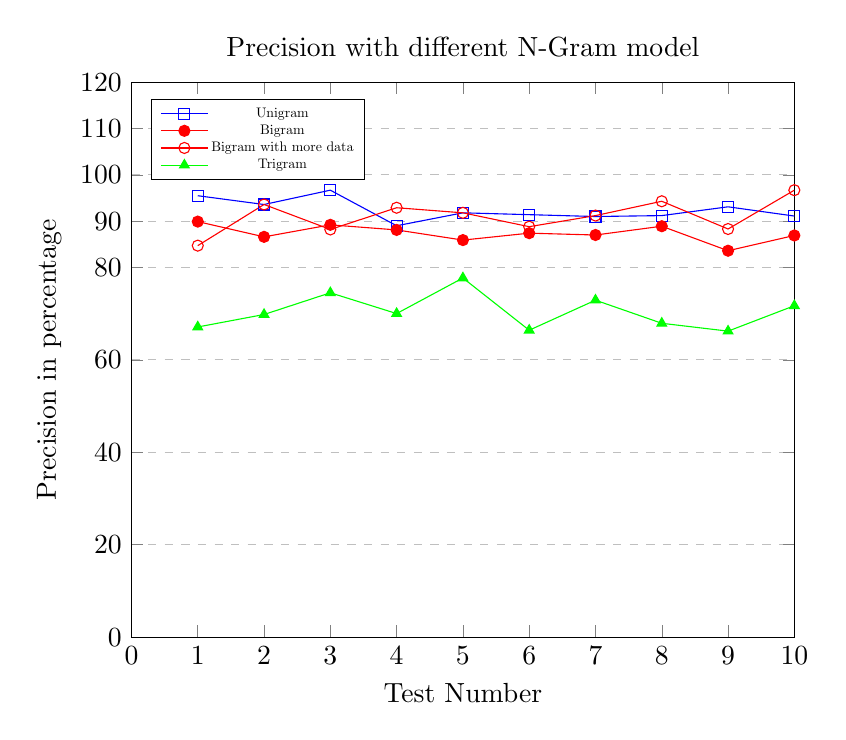
\begin{tikzpicture}
\begin{axis}[
    legend style={nodes={scale=0.5, transform shape}},
    % legend image post style={mark=*},
    title={Precision with different N-Gram model},
    xlabel={Test Number},
    ylabel={Precision in percentage},
    xmin=0, xmax=10,
    ymin=0, ymax=120,
    xtick={0,1,2,3,4,5,6,7,8,9,10},
    ytick={0,20,40,60,80,90,100,110,120},
    legend pos=north west,
    ymajorgrids=true,
    grid style=dashed,
]

\addplot[
    color=blue,
    mark=square,
    % legend = "Unigram"
    ]
    coordinates {
    (1,95.5)(2,93.6)(3,96.7)(4,89)(5,91.8)(6,91.4)(7,91.0)(8,91.2)(9,93.1)(10,91.1)
    };
    \legend{Unigram};
\addplot[
    color=red,
    mark=*,
    ]
    coordinates {
    (1,89.9)(2,86.6)(3,89.2)(4,88.1)(5,85.9)(6,87.4)(7,87)(8,88.9)(9,83.6)(10,86.9)
    };

    \addlegendentry{Bigram};
\addplot[
    color=red,
    mark=o,
    ]
    coordinates {
    (1,84.7)(2,93.6)(3,88.2)(4,92.9)(5,91.8)(6,88.8)(7,91.2)(8,94.3)(9,88.3)(10,96.7)
    };

    \addlegendentry{Bigram with more data};
\addplot[
    color=green,
    mark=triangle*,
    ]
    coordinates {
    (1,67.1)(2,69.8)(3,74.5)(4,70)(5,77.7)(6,66.4)(7,72.9)(8,67.9)(9,66.2)(10,71.7)
    };

    \addlegendentry{Trigram};
    
    
\end{axis}
\end{tikzpicture}
\end{center}
\newline


In terms of precision, unigram, as suggested in the chart, has the highest number of accuracy(92.44\%). Bigram trained with a larger data set is placed as the second place with the accuracy of (91.05\%). Bigram has the third highest accuracy(87.35\%) and trigram has the lowest accuracy(70.42\%). 
\newline
\begin{center}
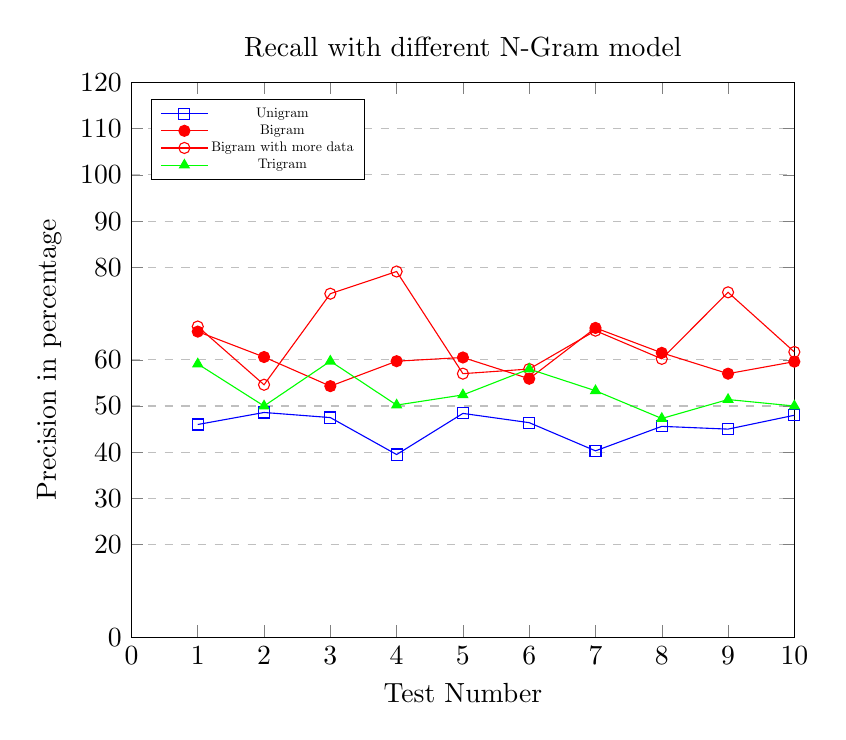
\begin{tikzpicture}
\begin{axis}[
    legend style={nodes={scale=0.5, transform shape}},
    % legend image post style={mark=*},
    title={Recall with different N-Gram model},
    xlabel={Test Number},
    ylabel={Precision in percentage},
    xmin=0, xmax=10,
    ymin=0, ymax=120,
    xtick={0,1,2,3,4,5,6,7,8,9,10},
    ytick={0,20,30,40,50,60,80,90,100,110,120},
    legend pos=north west,
    ymajorgrids=true,
    grid style=dashed,
]

\addplot[
    color=blue,
    mark=square,
    % legend = "Unigram"
    ]
    coordinates {
    (1,46)(2,48.6)(3,47.5)(4,39.5)(5,48.4)(6,46.4)(7,40.3)(8,45.6)(9,45)(10,48)
    };
    \legend{Unigram};
\addplot[
    color=red,
    mark=*,
    ]
    coordinates {
    (1,66.1)(2,60.6)(3,54.3)(4,59.7)(5,60.5)(6,55.9)(7,66.9)(8,61.5)(9,57)(10,59.6)
    };

    \addlegendentry{Bigram};
\addplot[
    color=red,
    mark=o,
    ]
    coordinates {
    (1,67.2)(2,54.6)(3,74.3)(4,79.1)(5,57)(6,58)(7,66.3)(8,60.2)(9,74.6)(10,61.7)
    };

    \addlegendentry{Bigram with more data};
\addplot[
    color=green,
    mark=triangle*,
    ]
    coordinates {
    (1,59.1)(2,50)(3,59.7)(4,50.2)(5,52.4)(6,58)(7,53.3)(8,47.3)(9,51.4)(10,50)
    };

    \addlegendentry{Trigram};
    
    
\end{axis}
\end{tikzpicture}
\end{center}
\newline


In terms of recall, we can see that the bigram trained by a larger data set has the overall highest accuracy(65.3\%). Bigram model is placed at the second place with the accuracy of (60.21\%).Trigram has the third highest accuracy(53.41\%). with some cases that are higher or equal to bigram. Unigram has lower accuracy(45.53\%).
\newline
\begin{center}
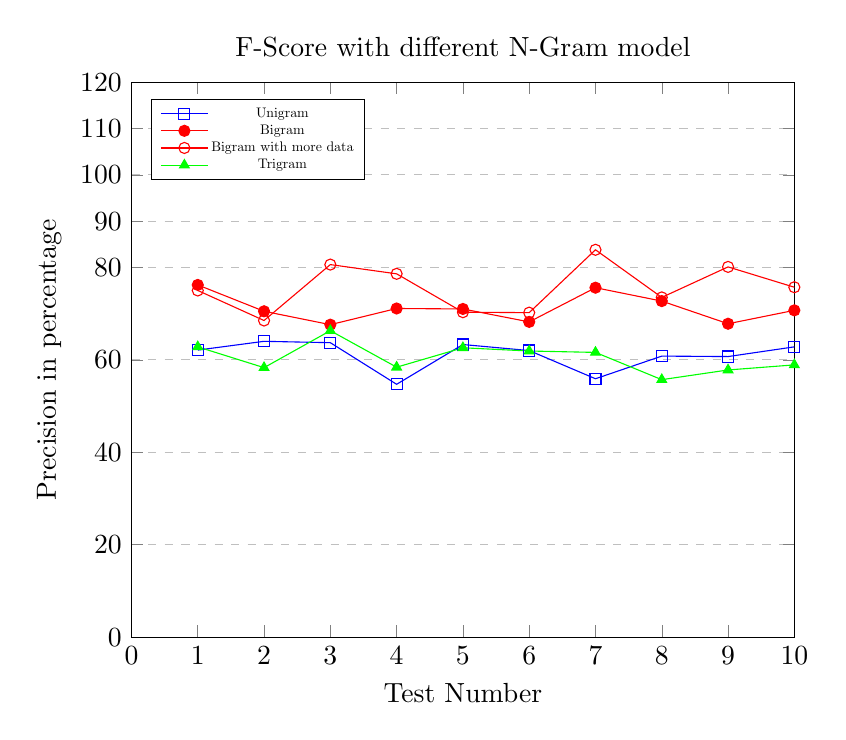
\begin{tikzpicture}
\begin{axis}[
    legend style={nodes={scale=0.5, transform shape}},
    % legend image post style={mark=*},
    title={F-Score with different N-Gram model},
    xlabel={Test Number},
    ylabel={Precision in percentage},
    xmin=0, xmax=10,
    ymin=0, ymax=120,
    xtick={0,1,2,3,4,5,6,7,8,9,10},
    ytick={0,20,40,60,80,90,100,110,120},
    legend pos=north west,
    ymajorgrids=true,
    grid style=dashed,
]

\addplot[
    color=blue,
    mark=square,
    % legend = "Unigram"
    ]
    coordinates {
    (1,62.1)(2,64)(3,63.7)(4,54.7)(5,63.3)(6,62)(7,55.9)(8,60.8)(9,60.7)(10,62.8)
    };
    \legend{Unigram};
\addplot[
    color=red,
    mark=*,
    ]
    coordinates {
    (1,76.2)(2,70.5)(3,67.6)(4,71.1)(5,71)(6,68.2)(7,75.6)(8,72.7)(9,67.8)(10,70.7)
    };

    \addlegendentry{Bigram};
\addplot[
    color=red,
    mark=o,
    ]
    coordinates {
    (1,75)(2,68.5)(3,80.6)(4,78.6)(5,70.3)(6,70.2)(7,83.8)(8,73.5)(9,80.1)(10,75.7)
    };

    \addlegendentry{Bigram with more data};
\addplot[
    color=green,
    mark=triangle*,
    ]
    coordinates {
    (1,62.8)(2,58.3)(3,66.3)(4,58.4)(5,62.6)(6,61.9)(7,61.6)(8,55.7)(9,57.8)(10,58.9)
    };

    \addlegendentry{Trigram};
    
    
\end{axis}
\end{tikzpicture}
\end{center}
\newline


In terms of F-score, we can see that biogram trained with a larger data set have the highest number of accuracy(75.63\%) Bigram model is placed at the second place with the accuracy of (71.14\%).Trigram has the third highest accuracy(61\%). with some cases that are higher or equal to bigram. Unigram has lower accuracy(60.43\%).
\newline
\begin{center}
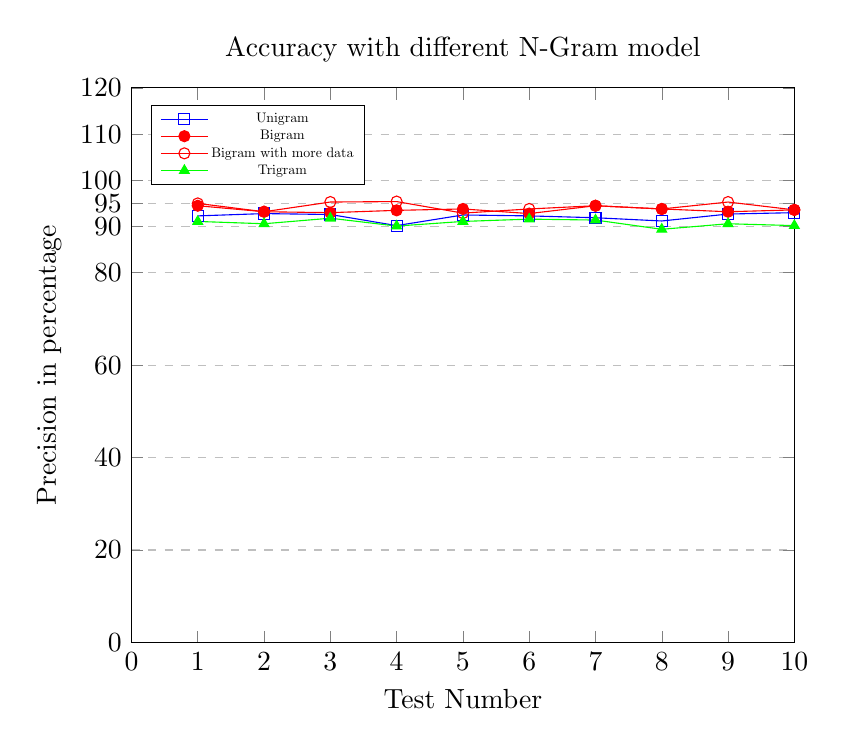
\begin{tikzpicture}
\begin{axis}[
    legend style={nodes={scale=0.5, transform shape}},
    % legend image post style={mark=*},
    title={Accuracy with different N-Gram model},
    xlabel={Test Number},
    ylabel={Precision in percentage},
    xmin=0, xmax=10,
    ymin=0, ymax=120,
    xtick={0,1,2,3,4,5,6,7,8,9,10},
    ytick={0,20,40,60,80,90,95,100,110,120},
    legend pos=north west,
    ymajorgrids=true,
    grid style=dashed,
]

\addplot[
    color=blue,
    mark=square,
    % legend = "Unigram"
    ]
    coordinates {
    (1,92.3)(2,92.8)(3,92.6)(4,90.2)(5,92.5)(6,92.3)(7,91.9)(8,91.2)(9,92.7)(10,93)
    };
    \legend{Unigram};
\addplot[
    color=red,
    mark=*,
    ]
    coordinates {
    (1,94.5)(2,93.2)(3,93)(4,93.5)(5,93.8)(6,92.8)(7,94.5)(8,93.8)(9,93.2)(10,93.6)
    };

    \addlegendentry{Bigram};
\addplot[
    color=red,
    mark=o,
    ]
    coordinates {
    (1,95)(2,93.2)(3,95.3)(4,95.4)(5,92.9)(6,93.8)(7,94.5)(8,93.8)(9,95.3)(10,93.6)
    };

    \addlegendentry{Bigram with more data};
\addplot[
    color=green,
    mark=triangle*,
    ]
    coordinates {
    (1,91.1)(2,90.6)(3,91.8)(4,90.1)(5,91.1)(6,91.6)(7,91.4)(8,89.4)(9,90.6)(10,90.2)
    };

    \addlegendentry{Trigram};
    
    
\end{axis}
\end{tikzpicture}
\end{center}


In terms of accuracy, we can see that biogram trained with a larger data set have the highest number of accuracy(94.28\%) Bigram model is placed at the second place with the accuracy of (93.59\%).Unigram has the third highest accuracy(92.15\%). with some cases that are higher or equal to bigram. Trigram has lower accuracy(90.79\%).

The question comes to why trigram behaves poorly in comparison with unigram and bigram, not to mention bigram trained with a large data set. One of the major factors is the data set and length of messages. Since trigram separates the sentence by three words, it would work better with messages that are longer. Evidentfully, trigram with recall but poorly with precision. This means that they have a higher number of false negatives but lower numbers of false positives. Such result is an indication that spam filters with trigram trained by this dataset have higher chance to misclassify some messages as spam messages. This behavior is not ideal since the cost of misplacing normal messages into spam filters is relatively expensive compared to the unigram model which will be discussed in the following paragraphs.


As the result shows, trigram works relatively well in correctly classifying messages. However, due to the nature of trigram, some tokens in the test set were not encountered in the training set. Even with the help of good-turning smoothing, it behaves poorly when strange words are encountered. The good side is that with words that the model has encountered, trigram has the highest number of accuracy. On the other hand, unirgram behaves relatively well in precision, but it behaves terribly in recall. This is an indication that algorithms implemented with unigram have a higher number of false negatives but lower number of false positives. This means that unigram is easier to misclassify as ham messages. Such action, even though not desirable, is still acceptable since it would be worse to place emails into spam folders. The reason for this is that unigram only counts the occurrence for a single word and calculates the frequency of a word against the whole train set. 
The F-score is a way to compare both precision and recall. As suggested in the chart, spam filters with trigram and unigram works appropriately the same. The difference between them and bigram is approximately 10\%. It’s safe to say that bigram, when trained by this particular training set, produces a lower number of false positives and lower number of false negatives. 


There are many factors that play an important role in arriving at this result. One of the most important factors is the size and length of training data. Due to the fact that there are many occurrences of tokens trigram models have never encountered, such as strange combinations of words or out of dictionary words, trigram model works even worse than simple unigram model. However, the training data set is sufficient for bigram models in terms of size and length. Thus, also as the result suggested, produces the highest number overall accuracy in comparison with bigram and trigram. The difference between bigram and unigram is approximately 1.5\% and difference between bigram and trigram is approximately 3.5\%. Such hypothesis is also validated through my experiment with bigram trained by a larger data set. Even though the length of the training data set is increased, the size of training data increased by approximately 10\%/. The difference between accuracy for bigram and accuracy for bigram trained with a large data set varies by 0.69\%. Such an increase does not seem like a big deal but keep in mind that we only added 500 examples to the training set. With bigger size of training data, the accuracy for naive bayes classifiers with bigram models can increase to at least 95\%.
Even though the time for training is increasing exponentially, it’s still worthwhile since future users will not need to train the model every time they use it. 

\section{Conclusion:}

Spam filtering is a challenging and complex problem that requires integration of many methods and techniques. Many methods have been invented and implemented by the leading company in the technology industry. Those methods include but are not limited to traffic tracking filtering, white-list and black-list, support vector machine and naive bayes classifier. On top of that, many methods are invented to target certain parts of the spam messages, such as link filtering, header filtering and content filtering. All those parts work together to create a state of art cutting edge spam filter that we are using right now. 


Spam filtering, or more specifically, content based spam filtering that deploys naive bayes classification with N-gram have potential to accurately classify spam messages under the assumption that the size and length of the training set is sufficient.  This article validates that natural language processing techniques can be deployed to improve the overall accuracy of spam filtering programs. As the result section suggests, a spam filter that deploys naive bayes classification with bigram yields 93.59\% of overall accuracy, which has a significant increase of 1.5\% compared with simple unigram implementation.  When the bigram model is trained with 90\% of data, we can see that the accuracy of validation increases by 0.69\%. Such result validates the hypothesis that the accuracy of spam filters that implement naive bayes classifier and N-gram model have potentials that are not yet fully exploited. 


This experiment is limited since the dataset is not sufficient in length or in size. The Natural language processing techniques are not sophisticatedly implemented. With the help of advanced smoothing algorithms, I believe that the baseline of accuracy can increase significantly. 
Feature work on this topic would be to study how important smoothing algorithms and the size of database is for spam filters. Feature researchers should implement better smoothing algorithms and 5 or more gram models. Using a large dataset to train the model and study how data size, message length would affect the performance of spam filters. 

\newpage
\medskip

\bibliographystyle{unsrt}%Used BibTeX style is unsrt
\bibliography{sample}
\end{document}